\chapter{Controller Design}\label{chap:Control}
The system of the quadcopter has been described by a mathematical model, that is to be used in the design of a control system. The control system must stabilize the unstable system of the quadcopter. It should also meet the functional requirements stated in \autoref{ch:functionalRequirements}.

The model is divided into two submodels, an attitude model and a translational one. It is therefore desirable to design two control systems, one for each one. The attitude controller constitutes an inner loop surrounded by the translational x and y controllers, and the z controller handles the amount of thrust applied by the motors changing the retired sum of their rotational speeds. \autoref{fig:ControlHeadDiagram} shows the relation between the different controllers in the system.
%
\begin{figure}[H]
	\centering
	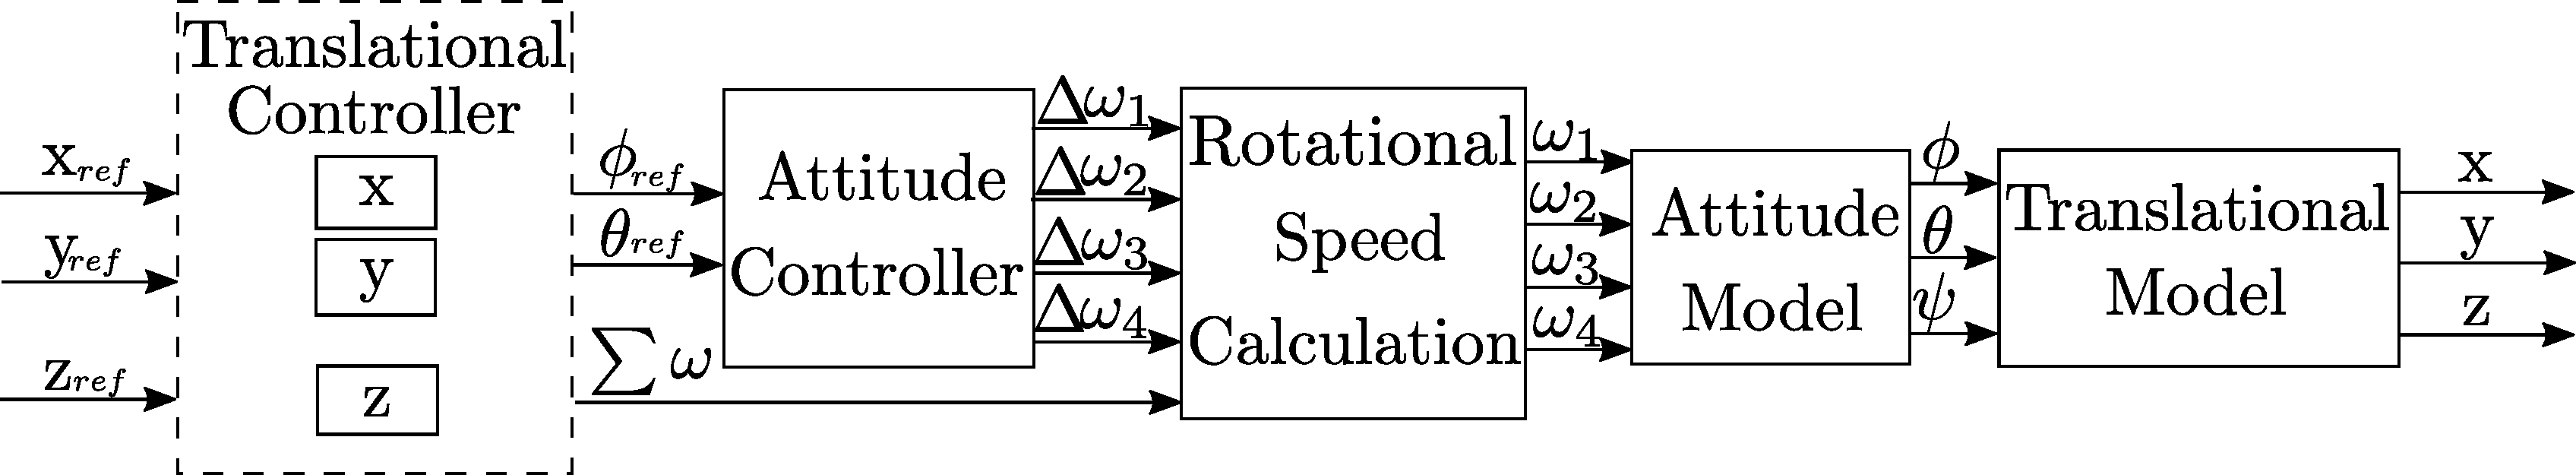
\includegraphics[width=1 \textwidth]{figures/generalcontroldiagram}
	\caption{Block diagram of overall control system.}
	\label{fig:ControlHeadDiagram}
\end{figure}

The attitude controller is an inner controller and it is designed using a state space approach  \cite{ssReference}. The translational control system is designed with classical control methods, such as bode plots and root locis. The rotational speed calculator takes into account the rotational speeds that the attitude controller needs in each motor and the sum that is needed to get the desired thrust in the $z_\mathrm{I}$ direction. Then, it combines both to give the final control action that is applied to the system.

First the design of the attitude controller is done followed by the design of the translational controller. When the controllers are designed, they are simulated with the models to ensure, that the controllers yield the desired behavior, as these represent the true behavior of the plant. If the controllers yield an acceptable outcome, they are to be implemented in the system. To do so, they are first discretized. It is necessary to simulate the discrete controllers and compare the results with the continuous controllers, as some design considerations may be lost in the discretization. Lastly the controllers are implemented on the micro controller and the system is to be tested in the Vicon room. 